\documentclass[../main.tex]{subfiles} 
\begin{document}
\chapter{Conclusie}

\section{Beveiliging in de softwarecyclus}
kwetsbaarheden kunnen binnensluipen in elk van de softwareontwikkelingsstadia. Het is dan ook belangrijk de soorten aanvallen te kunnen onderscheiden en te weten welke tegenmaatregelen te treffen in elke situatie en fase van de ontwikkeling. Deze cursus heeft zich voornamelijk toegelegd op het implementatieniveau en af en toe het designniveau.

Het inpassen van tegenmaatregelen betekenen echter niet dat er een complete verandering nodig is in het ontwikkelingsproces. Aan de hand van \textbf{touchepoints} en \textbf{software process enrichtments} kunnen deze twee worden gecombineerd. Enkele voorbeelden zijn \textit{Cigital's touchepoints} en \textit{Microsoft's SDL}.

\section{Bedreigingsmodellering}
Het modelleren van bedreigingen is een activiteit die plaatsvindt in de beginfase van de softwareontwikkelingslevenscyclus. Het centrale doel is een goed zicht krijgen op de mogelijke kwetsbaarheden van het systeem dat wordt ontwikkeld. 

Het modelleren kan gebeuren op verschillende niveaus van abstractie:
\begin{itemize}
	\item \textbf{Systeemniveau} \\ \textit{Bv. bedreigingsmodellering van het internet e-mails systeem.}
	\item \textbf{Applicatie- of componentniveau} \\ \textit{Bv. bedreigingsmodellering van de e-mail client software.}
\end{itemize}
\noindent
Kwetsbaarheden kunnen worden onderverdeeld in categorie\"en:
\begin{itemize}
	\item \textbf{S}poofing
	\item Information \textbf{T}ampering
	\item \textbf{R}epudiation
	\item \textbf{I}nformation disclosure
	\item \textbf{D}enial of service
	\item \textbf{E}levation of privilege
\end{itemize}
Wanneer bedreigingen aan het licht worden gebracht is het belangrijk dat we een goed begrip hebben van de \textit{assets} en van de bedreigingsagent, meer bepaald wat dienst motivatie en sterkte is.

Microsoft heeft als onderdeel van het \textit{Secure Development Life Cycle} een bedreigingsmodelleringsactiviteit gedefinieerd. Aan de hand van documentatie en met gebruik van tools kunnen bedreigingen in kaart worden gebracht. Aan de hand van een voorbeeld uit dit boek zullen we het proces illustreren.

\subsection{Define Use Scenarios}
Allereerst moet gedefinieerd worden hoe het systeem gebruikt zal worden en hoe niet. Dit zorgt ervoor dat de discussie rond bedreigingsmodellering duidelijk omgrensd wordt. We vragen ons af welke scenario's binnen de strekking van het programma liggen. Bijvoorbeeld: houden we rekening met bedreigingen van interne agenten?

\subsection{List External Dependencies}
Elke applicatie steunt op infrastructurele software om correct te functioneren. Het is belangrijk om deze goed te documenteren. Nemen we als voorbeeld een winkel voor huisdieren. Deze steunt op:
\begin{multicols}{2}
\begin{itemize}
	\item Web-based client
	\item Browser
	\item Windows Server
	\item Microsoft ISS
	\item SQl Server 
	\item .NET Framework
\end{itemize}
\end{multicols}

\subsection{Define Security Assumptions}
Welke beveiligingsgaranties verwachten we van onze externe afhankelijkheden? Voor de huisdierenwinkel:
\begin{itemize}
	\item ISS en ASP.NET voorzien authenticatie
	\item Fysieke toegang tot de server is beperkt tot beheerders
	\item Configuratiebestanden worden beschermt door het besturingssysteem
\end{itemize}

\subsection{Create External Security Notes}
Documenteer beveiligingsrelevante informatie voor de gebruikers van de applicatie.
\begin{figure}[h1]
    \centering
    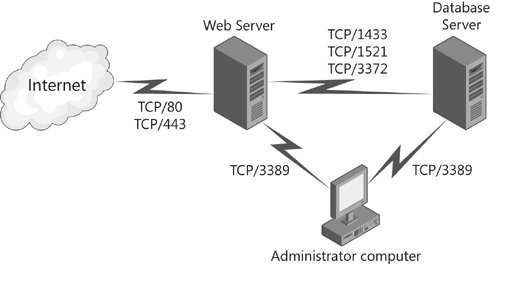
\includegraphics[width=0.6\textwidth]{../images/external_security_notes.png}
    \caption{External Security Notes}
    \label{fig:external_security_notes}
\end{figure}

\subsection{Model the Application}
Modelleer het systeem aan de hand van \textit{dataflow} diagrammen. Typisch worden volgende zaken gemodelleerd:
\begin{multicols}{2}
\begin{itemize}
	\item Externe entiteiten
	\item Processen
	\item Dataopslag
	\item Datastroom
	\item Beperkingen privileges
\end{itemize}
\end{multicols}

\begin{figure}[h!]
    \centering
    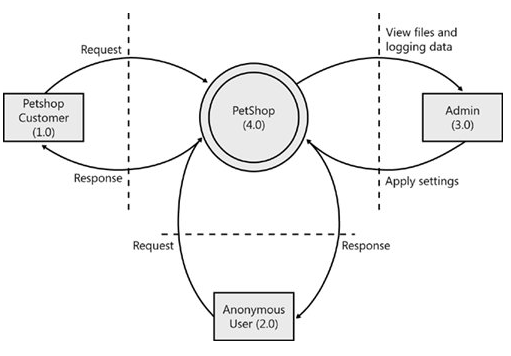
\includegraphics[width=0.6\textwidth]{../images/pet_shop_model_1.png}
    \caption{Voorbeeldmodel}
    \label{example1}
\end{figure}

\begin{figure}[h!]
    \centering
    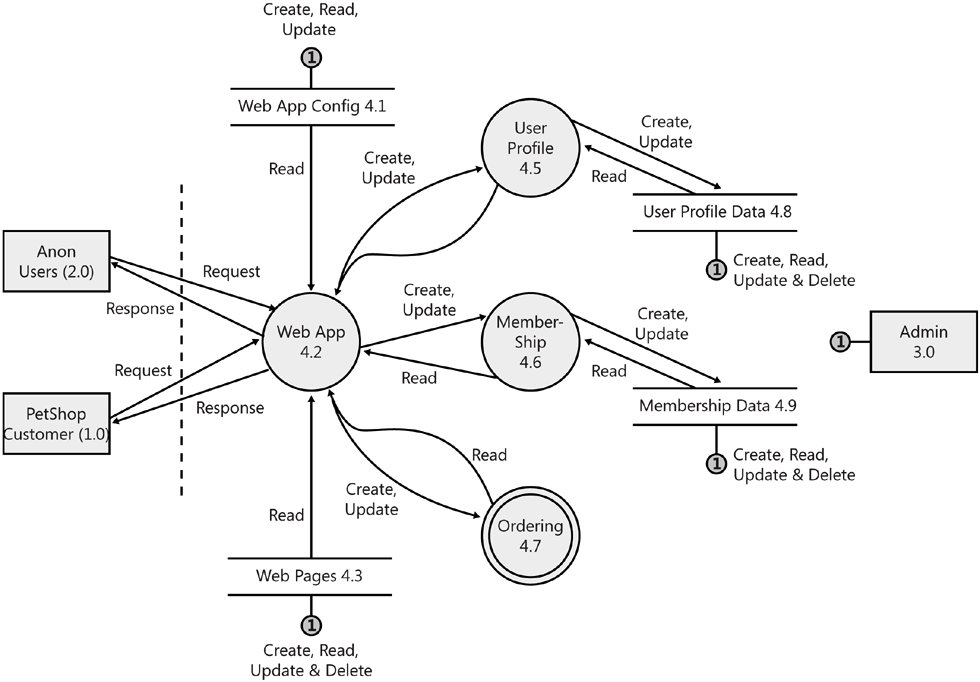
\includegraphics[width=0.8\textwidth]{../images/pet_shop_model_2.png}
    \caption{Voorbeeldmodel}
    \label{example2}
\end{figure}

\begin{figure}[h!]
    \centering
    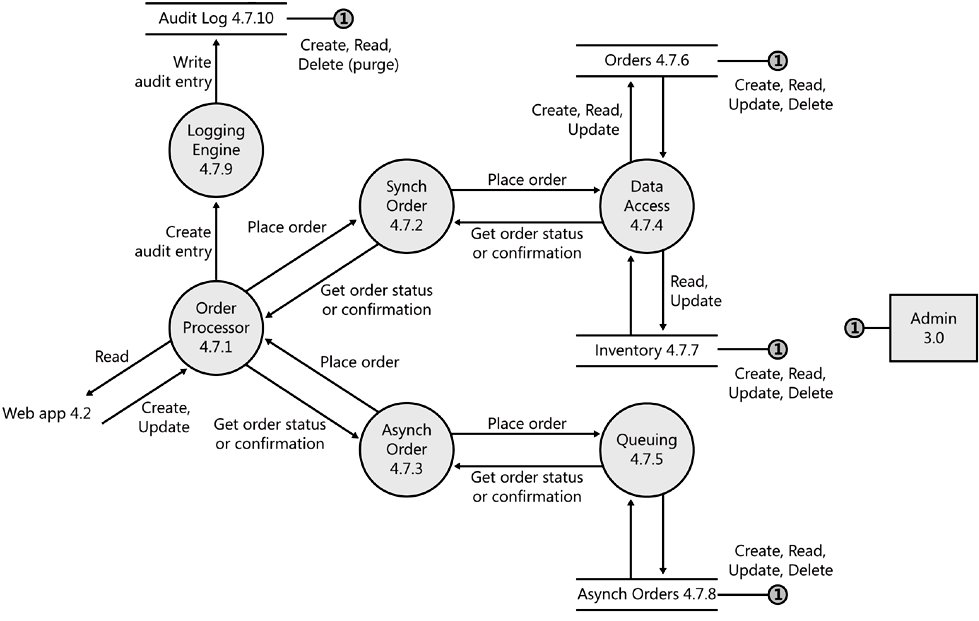
\includegraphics[width=0.8\textwidth]{../images/pet_shop_model_3.png}
    \caption{Voorbeeldmodel}
    \label{example3}
\end{figure}

\subsection{Determine Threat Types}
Microsofts proces maakt gebruikt van de  \textbf{STRIDE} bedreigingstypen. (zie eerder) 
\subsection{Identify Threats}
Alle DFD elementen worden beschouwd als \textit{assets}. Zie afbeeldinge \ref{STRIDE}.
\begin{figure}[h!]
    \centering
    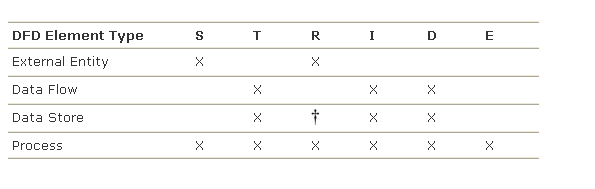
\includegraphics[width=0.8\textwidth]{../images/STRIDE.png}
    \label{STRIDE}
    \caption{DFD en STRIDE}
\end{figure}
\subsection{Determine Risk}
Subjectieve numerieke methodes om het belang te schatten (bv. DREAD) worden niet meer gebruikt. De huidige guideline zegt gebruik te maken van objectieve karakteristieken zoals:
\begin{itemize}
	\item Server applicatie versus client applicatie
	\item Lokaal versus toegankelijk op afstand
	\item Toegankelijk voor anonieme gebruikers
\end{itemize}

\begin{figure}[h!]
    \centering
    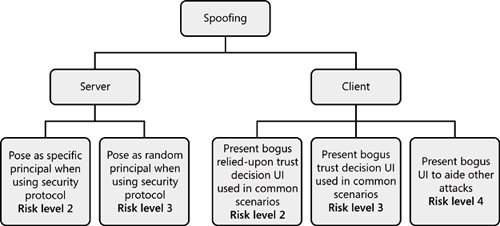
\includegraphics[width=0.8\textwidth]{../images/spoofing.png}
    \caption{Spoofing}
    \label{spoofing}
\end{figure}

\begin{figure}[h!]
    \centering
    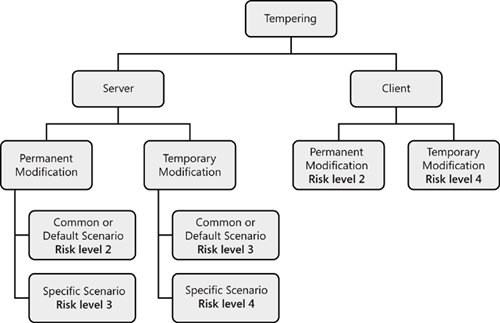
\includegraphics[width=0.8\textwidth]{../images/tampering.png}
    \caption{Tampering}
    \label{tampering}
\end{figure}
    
\begin{figure}[h!]
    \centering
    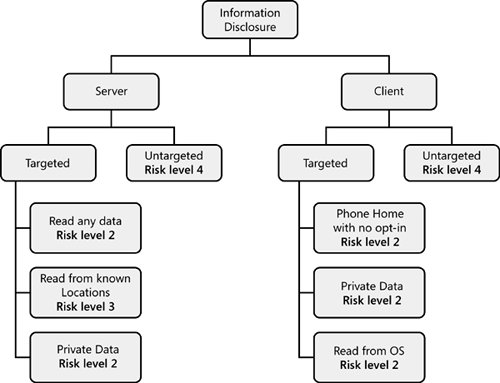
\includegraphics[width=0.8\textwidth]{../images/information.png}
    \caption{Information Disclosure}
    \label{information}
\end{figure}
    
\begin{figure}[h!]
    \centering
    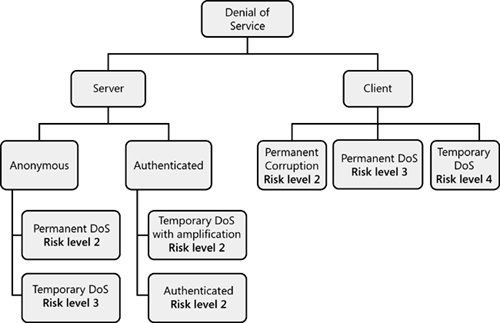
\includegraphics[width=0.8\textwidth]{../images/dos.png}
    \caption{Denial of Service}
    \label{dos}
\end{figure}
    
\begin{figure}[h!]
    \centering
    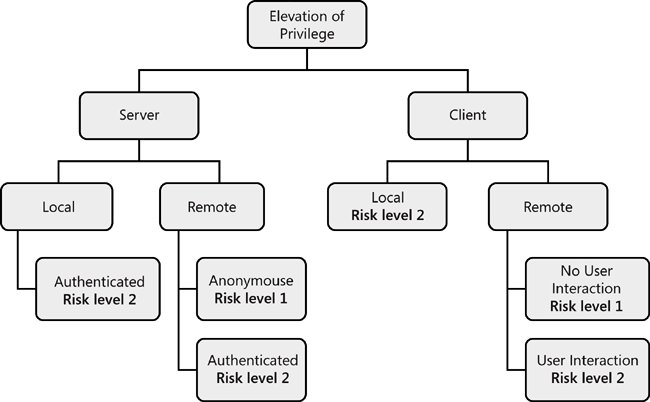
\includegraphics[width=0.8\textwidth]{../images/eop.png}
    \caption{Elevation of Privileges}
    \label{eop}
\end{figure}

\subsection{Plan Mitigations}
Strategie\"en:
\begin{itemize}
	\item Niets doen
	\item De feature verwijderen
	\item De feature uitschakelen
	\item De gebruiker waarschuwen (\textit{dancing pigs syndrome})
	\item Weerstand bieden met technologie
\end{itemize} 

We kunnen concluderen dat bedreigingsmodellering  plaatsvindt in de vroege fasen van de software levenscyclus. Dit is de fase waarin bedreigingprofiel duidelijk wordt en er tegenmaatregelen kunnen worden getroffen op een ge\"informeerde manier. 
\\\\
Microsoft plaats \textit{Bedreigingsmodellering} op plaats 2 in de de lijst van belangrijkste veiligheidsgerelateerde activiteiten. Op de eerste plaatst staat statische analyse van implementatiekwetsbaarheden.

\section{Principes, patronen en richtlijnen}
Kennis en ervaring verkregen in het ontwikkelen van veilige software het geleid tot een verzameling zogenaamde \textit{best practices}. 
\begin{itemize}
	\item \textbf{Principes} zijn generische richtlijnen, toepasbaar doorheen heel de ontwikkelingscyclus.
	\item \textbf{Patronen} zijn herbruikbare oplossing voor veiligheidsproblemen op architecturaal niveau.
	\item \textbf{Richtlijnen} bieden een specifiek richtsnoer over hoe wel en niet te programmeren in zekere programmeertalen. 
\end{itemize}

\subsection{Principes}
\begin{itemize}
	\item \textbf{Simplicity} \\ 
	\textit{Economy of mechanism}: Eenvoudige tegenmaatregelen zijn eenvoudiger juist te krijgen en eenvoudiger te begrijpen.
	\item \textbf{Open Design} \\
	Inzetten op beveiliging zelfs al weet de aanvaller wat de tegenmaatregelen zijn. Dus geen  \textit{security by obscurity}.
	\item \textbf{Least Privilege} \\ 
	Elk onderdeel van het systeem mag niet meer rechten hebben dan nodig is voor diens functie uit te voeren.
\end{itemize}

\subsection{Patronen}
\subsubsection{Architectuurpatronen}
\begin{itemize}
	\item \textbf{Compartimentering} \\ Ontwerp het systeem zo dat inbreuken worden afgeschermd.
	\item \textbf{Minimaliseer het aanvalsoppervlak} \\ Reduceer de hoeveelheid interfaces en informatie toegankelijk voor aanvallers. Maak hiervoor eventueel gebruik van een \textit{secure service facade}.
	\item \textbf{Complete Mediation} \\ Ontwerp het systeem zo dat elke toegang gebeurt langs een vorm van validatie. Gebruik hiervoor authenticatie of afdwingen toegangscontrole.
\end{itemize}

\subsubsection{Ontwerppatronen}
\begin{itemize}
	\item \textbf{Security Association} \\
	Definieer een container datastructuur die de data groepeert die gebruikt wordt door \'e\'en deelnemer in beveiligde communicatie.
	\item \textbf{Security context} \\
	Definieer een container datastructuur die groepsgerelateerde attributen van de principal of het proces groepeert.
	\item \textbf{Role-based access} \\
	Ontkoppel identiteiten van gebruikers van hun privileges.
	\item \textbf{Limited view} \\
	Maak de gebruikersinterface op zo'n manier dat gebruikers enkel zien wat ze mogen zien.
\end{itemize}

\subsection{Richtlijnen}
Er zijn zoveel richtlijnen, waarvan vele vaag, wat betekent dat de programmeur ze niet allemaal in het achterhoofd kan houden. Een vari\"eteit aan statische analysetools kunnen (een deel) van deze richtlijnen controleren. Voorbeelden hiervan zijn \textit{Coverity, Fortify, FxCop, FindBugs}.
\subsubsection{Voor C}
\begin{itemize}
	\item \textbf{MEM00-C.} Allocate and free memory in the same module, at the same level of abstraction
	\item \textbf{MEM01-C.} Store a new value in pointers immediately after free()
	\item \textbf{MEM02-C.} Immediately cast the result of a memory allocation function call to a pointer to the allocated type
	\item \textbf{MEM06-C.} Ensure that sensitive data is not written out to disk
	\item \textbf{MEM09-C.} Do not assume memory allocation functions initialize memory
	\item \textbf{MEM10-C.} Define and use a pointer validation function
	\item \textbf{MEM11-C.} Do not assume infinite heap space
\end{itemize}
\subsubsection{Voor Java}
\begin{itemize}
	\item \textbf{OBJ00-J.} Limit extensibility of classes and methods with invariants
	\item \textbf{OBJ01-J.} Declare data members as private and provide accessible wrapper methods
	\item \textbf{OBJ03-J.} Do not mix generic with nongeneric raw types in new code
	\item \textbf{OBJ04-J.} Provide mutable classes with copy functionality to safely allow passing instances to untrusted code
	\item \textbf{OBJ05-J.} Defensively copy private mutable class members before returning their references
	\item \textbf{OBJ07-J.} Sensitive classes must not let themselves be copied
	\item \textbf{OBJ11-J.} Be wary of letting constructors throw exceptions	
\end{itemize}


\section{Conclusie}
Ontwikkeling van veilige software is een relatief nieuwe ingenieursdiscipline.  De gemeenschap is nog volop aan het leren hoe ze \textit{best practices} kunnen omzetten in herhaalbare en verifieerbare processen. Desondanks is er voldoende empirisch bewijs om de waarde van het modelleren van bedreigingen en statische analyse aan te tonen.


\end{document}